\section{Ancestry \& Class Overview}
\label{Section_AncestryClassOverview}


\subsection*{Beginner Combinations} 

For your first time playing, the sheer amount of options can eb overwhelming. We recommend these tried and tested options:\\
\begin{minipage}[t][7cm][t]{1\textwidth}
\begin{enumerate}
	\item \textbf{Human, Knight, Koloss} - Human grants you the best card in the game, "Smite". Your knight passive lets you see half your deck on turn 1 to execute a devastating first strike. Koloss keeps you alive. Level into more ranks of Koloss to survive better, or rank up into Knight to improve your turn 1.
	\item \textbf{Half Elf, Ranger, Bard} - This very potent combination lets you deal maximum damage. Half Elf and Bard make each attack more powerful while Ranger lets you hits with many small attacks. Choose Ranger ranks when leveling up to increase your damage further. Bard is for a more supportive playstyle.
	\item \textbf{Fae, Druid, Assassin} - Fae lets ou play every card as if it had ranged. Druid and Assassin let you heal your allies and stun your enemies. All this combines to let you shape the flow of battle and keep your teammates alive. Choosing more ranks of Assassin will let you deal significant damage yourself, while more ranks of Druid let you support better.
	\item \textbf{Dwarf, Berserker, Pyromancer} - Dwarves are naturally sturdy, which complements the damage-focussed Pyromancer and Berserker for a well rounded character.  Both Pyromancer and Berserker will offer more damage as you get higher ranks of them. 
	\item \textbf{Centaur, Sangromancer, Witch} - Centaurs let you use the damage that is usually wasted when finishing an enemy by redirecting it to an adjacent one. This combines well with the immense damage output of Sangromancer. The Witch's passive is used to heal back the life costs on Sangromancer cards. Sangromancer provides more damage when leveling up, so that path is recommended. 
\end{enumerate}
\end{minipage}

All  ancestries. classes, elements and mechanics re arranged into one large wheel.
Classes that are placed adjacent to each other will share their elements, mechanics and synergies. 

\begin{figure}[ht]

	\begin{minipage}[t][6.5cm][t]{1\textwidth}
		\centering
		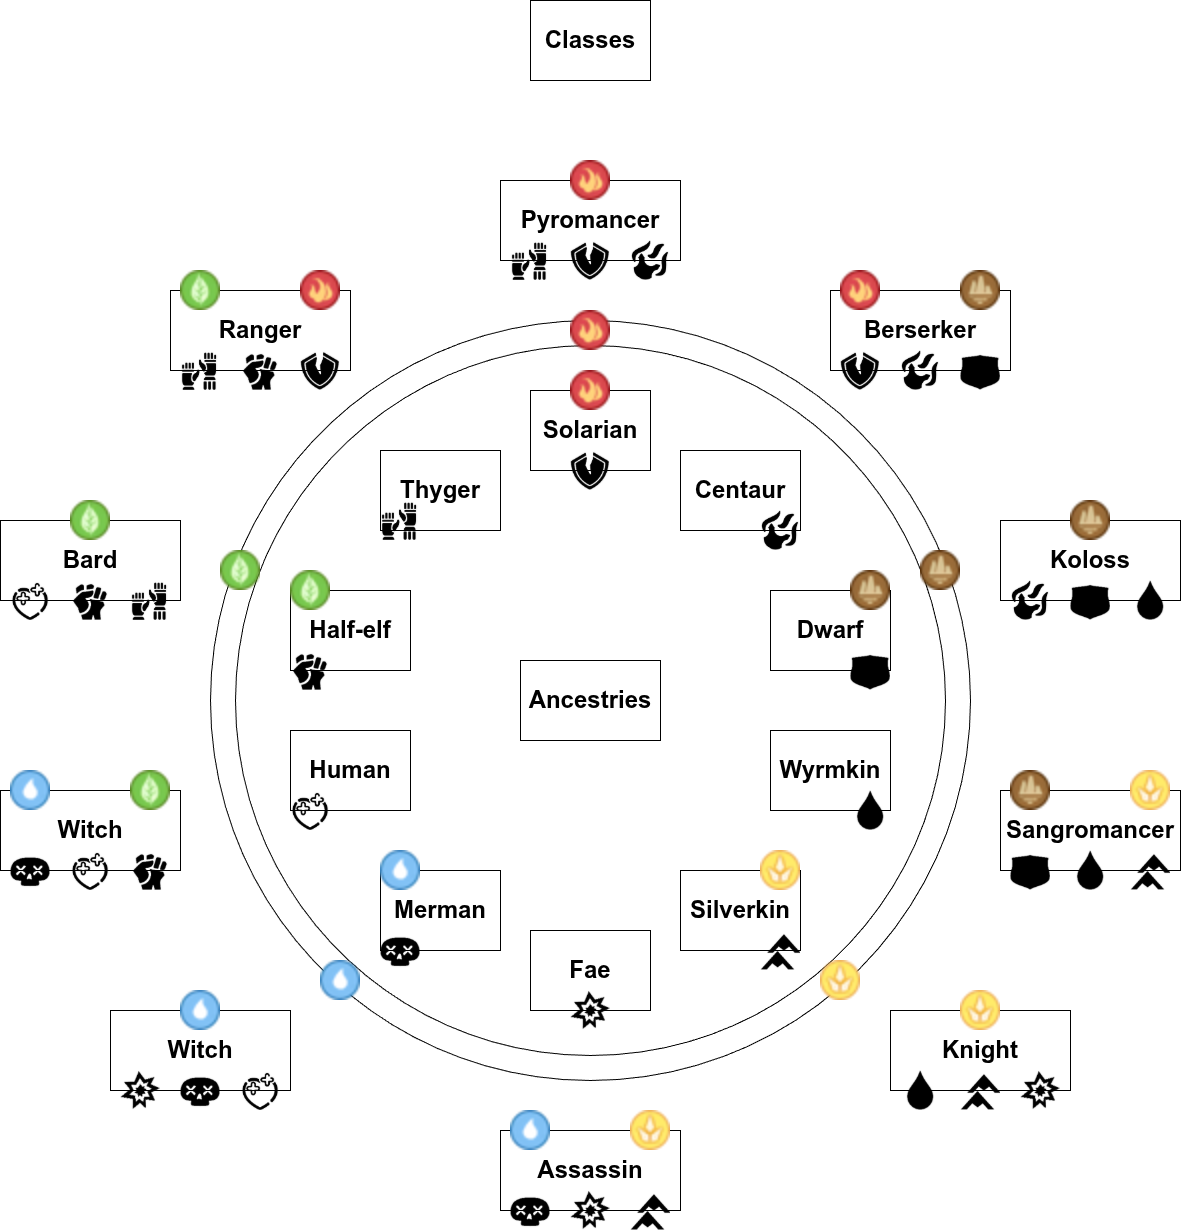
\includegraphics[width=0.9\linewidth, valign=t]{../GuidePics/Circle_Mechanics.drawio.png}
	\end{minipage}
\end{figure}
